\documentclass{article}
\usepackage[utf8]{inputenc}
\usepackage{amsmath}
\usepackage{siunitx}
\usepackage{graphicx}
\usepackage{float}
\title{ Report }
%\title{Report}
\author{Akshay Malige}
\date{February 2020}
\maketitle

\begin{document}

\begin{center}
Implementacja oprogramowania do testowania ukladow PASTTREC

Implementation of software for testing PASTTREC chips
\end{center}


\section*{Automatic Baseline alignment procedure}
Two of the most important parameters of the PASTTREC are gain and baseline uniformity.
High gain uniformity allows to treat all the channels equally, without the need of individual calibration procedures for the leading time and TOT measurements for each channel. The baseline level differs among the PASTTREC channels but it can be fine tuned thanks to the internal DAC circuits. In order to complete this task an automatic alignment procedure has been developed. The noise is registered as counts when the baseline is at the threshold position. Using the TRBnet interface the baseline of a channel is shifted by 2 mV at a time until the noise is registered. This gives the position of the baseline for a particular FEE channel. A python3 package has been developed which uses the TRBnet interface to align the baselines.

\subsection*{PASTTREC tools}

pasttrectools is a system-wide install-able application consist sing of two parts.
\begin{itemize}
  \item `pastrec.py` module with the interface
  \item user scripts
\end{itemize}

\subsection*{Requirements}
\begin{itemize}
  \item {python \geqslant	 3.5 }
  \item colorama
  \item setuptools
\end{itemize}

\subsection*{Installation}
\begin{itemize}
  \item python3 setup.py build
  \item sudo python3 setup.py install
\end{itemize}

\subsection*{Usage}

\begin{itemize}
  \item Asic's have to be reset after powering them on. This can be done using the \textbf{reset\_asic.py tdc\_id} (eg. reset\_asic.py 0x6400) 
  \item The communication with the asic's can be tested using the \textbf{communication\_test.py tdc\_id}
\end{itemize}

\subsection*{Baseline scan}
\begin{itemize}
  \item Use \textbf{baseline\_scan.py} script, see '--help' for usage and options details. Basic usage requires passage of TRBnet ids to scan : baseline\_scan.py 0x6400 0x6401 0x6402 0x6403 ...
\item Default execution will generate `result.json` file (JSON format file) which can be changed using `-o` option.
\item JSON output format.
\end{itemize}

\begin{figure}
\centering
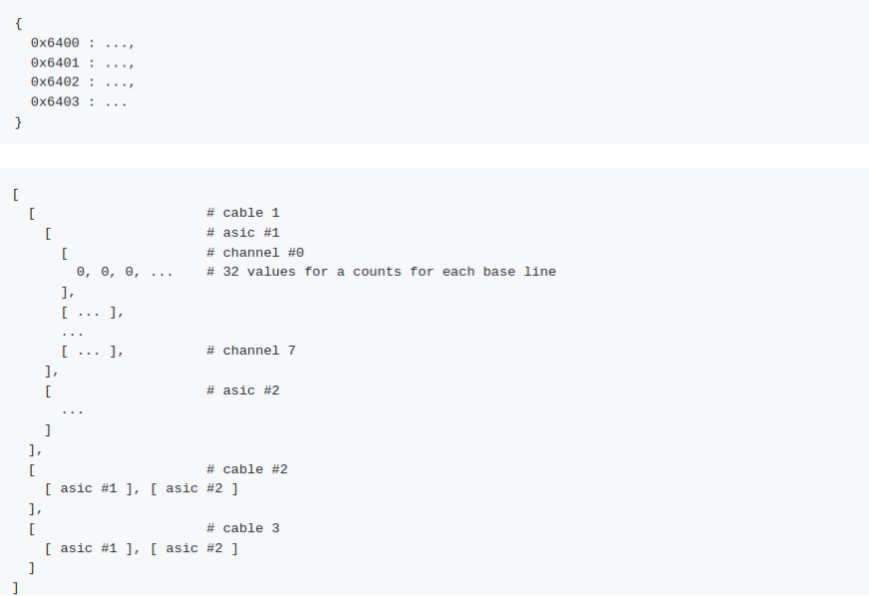
\includegraphics[width=10cm,height=8cm]{json_out.png}
\caption{Structure of the json output file from the baseline scan }
\end{figure}

The output contains a dictionary with a key being the TRBnet ids and values are multidimensional arrays of cables (2), asics(3), channels(8) and base line values (32) as shown in Figure 1.



\begin{itemize}
  \item Use \textbf{draw\_baseline\_scan.py} for drawing plots. Script requires one argument which is a json input file. e.g. ./draw\_baseline\_scan.py result.json
\end{itemize}

\subsection*{Extract baselines}
Use \textbf{calc\_baselines.py}, see '-h' for details. It allows to
\begin{itemize}
  \item Extract average baseline (weighted mean: 'bl = Sum\_i(ch\_i*cnt)/Sum(ch\_i)')
  \item Add offset for all channels (use '-blo val', where val is a number), if offset is not given, user will be asked for an offset for each chip.
  \item Dump registers to file, if '-D' then all registers, if '-d' then only baseline registers
  \item The json output contains a dictionary with a key being a TRBnet ids and values are next-level dictionaries of cables containing card info and asics and each asic dictionary has a list of PASTTREC registers and settings.
\end{itemize}
Example usage : ./calc\_baselines.py input.json -D output.dat -blo 0 -o output.json

\begin{itemize}
 \item The version in 'pasttrec.LIBVERSION' must be changed each time when structure/format of json data is changed.
\end{itemize}



\subsection*{Results}
The Time Over Threshold (TOT) spectra from radioactive source $^{55}$Fe is observed for 32 PASTTREC channels before and after the alignment procedure was applied in Figure 2. This procedure is very time efficient compared to the conventional method where the baselines are extracted by tuning the TOT spectra obtained from the straw channels. The other advantages are that the we don not need a functional detector to align the baselines and the result from the scans provide us with some additional information like the noise width and spread in the FEE's. Once the baseline configuration has been found, it remains stable over the time.
\begin{figure}[!ht]
\centering
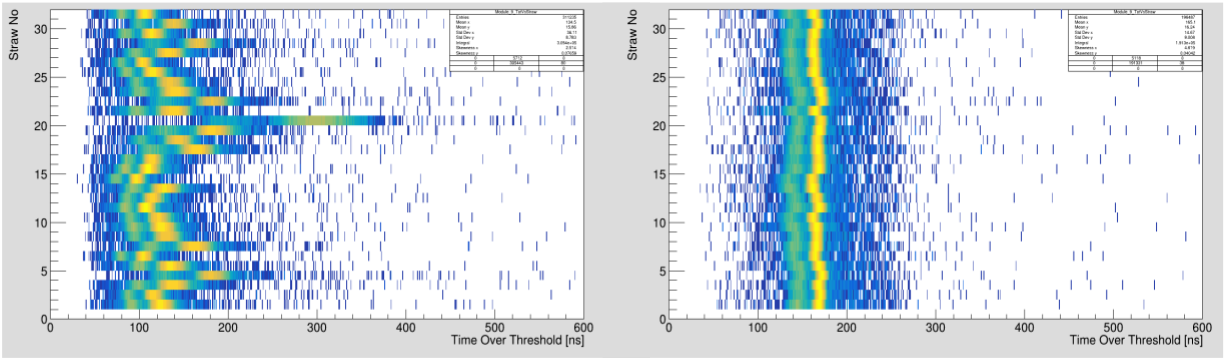
\includegraphics[width=12cm,height=5cm]{TOT_allignment.png}
\caption{Left: TOT spectrum versus straw channel for selected channels of the detector
before the baseline tune was applied. Right: TOT spectra after baseline scan and alignment procedure has been applied.}
\end{figure}

\end{document}
